% Chapter 1

\chapter{Introducción general} % Main chapter title

\label{Chapter1} % For referencing the chapter elsewhere, use \ref{Chapter1} 
\label{IntroGeneral}

Este capítulo presenta una visión general de los sistemas de gestión y
monitoreo en invernaderos, se abordan los desafíos actuales y las oportunidades
de mejora en el ámbito de la agricultura. Se describe la problemática
relacionada con la falta de optimización en los sistemas de cultivo
tradicionales. Además, se describen la motivación, los objetivos, el alcance y
los requerimientos asociados a los diferentes componentes del sistema.

%----------------------------------------------------------------------------------------

% Define some commands to keep the formatting separated from the content 
\newcommand{\keyword}[1]{\textbf{#1}}
\newcommand{\tabhead}[1]{\textbf{#1}}
\newcommand{\code}[1]{\texttt{#1}}
\newcommand{\file}[1]{\texttt{\bfseries#1}}
\newcommand{\option}[1]{\texttt{\itshape#1}}
\newcommand{\grados}{$^{\circ}$}

%----------------------------------------------------------------------------------------

%\section{Introducción}

%----------------------------------------------------------------------------------------
\section{Problemática actual}

La agricultura enfrenta desafíos crecientes en la optimización de la
productividad y la eficiencia, especialmente en regiones con condiciones
climáticas adversas y variables. Según la FAO (del inglés, \textit{Food and Agriculture
      Organization of the United Nations}) \cite{GAPReport2016}, para el año 2050, se
estima que la población superará los 9 mil millones de personas, lo que
demandará un aumento del 60\code{\%} en la producción de alimentos. Para
abordar este desafío, es fundamental optimizar el uso del agua, mejorar la
productividad agrícola y fomentar prácticas que contribuyan a la sostenibilidad
ambiental.

Ante estos retos, los cultivos hidropónicos han surgido como una solución
prometedora debido a su capacidad para utilizar los recursos de manera más
eficiente. Entre sus principales ventajas se destacan la reducción en el
consumo de agua \cite{EficienciaAgua2014}, la posibilidad de cultivar durante
todo el año en entornos controlados y un aumento significativo en la
productividad, gracias a la mayor velocidad de crecimiento y rendimiento de los
cultivos.

En la provincia de Misiones, la producción hidropónica ha experimentado un
crecimiento notable en los últimos años \cite{HorticulturaMisiones2024},
\cite{HidroponiaMisiones2024}. No obstante, persisten desafíos en la gestión
eficiente de los recursos esenciales. Actualmente, la mayoría de los
productores emplean sistemas de control basados en temporizadores programables,
los cuales no consideran las variaciones ambientales. Esto implica la necesidad
de intervenciones manuales frecuentes y mediciones directas, limitando la
eficiencia del proceso.

La ausencia de un monitoreo en tiempo real impacta negativamente en la calidad
y el rendimiento de los cultivos, aumentando los costos operativos y afectando
la sostenibilidad ambiental debido a la implementación de prácticas poco
optimizadas.

%----------------------------------------------------------------------------------------

\section{Motivación}

La motivación de este trabajo radica en el desarrollo e implementación de un
sistema basado en IoT (del inglés, \textit{Internet of Things}) y de bajo costo, que
permite monitorear en tiempo real y controlar de manera remota los invernaderos
de la Facultad de Ciencias Forestales (FCF) de la Universidad Nacional de
Misiones (UNaM).

Este sistema posibilita el registro continuo de diversas variables de interés,
como temperatura ambiente, humedad relativa, dióxido de carbono ($CO_2$),
niveles de nutrientes, y consumo de agua y energía, entre otros. Los datos
generados están disponibles para docentes, estudiantes e investigadores, para
su uso en la realización de tesis, investigaciones y trabajos académicos.

Así, el trabajo no solo tiene un impacto directo en la producción, sino
también en la formación académica y el avance científico. Proporciona una
plataforma de datos para el análisis y el desarrollo de nuevas soluciones
tecnológicas, alineadas con las demandas actuales de sostenibilidad ambiental y
seguridad alimentaria \cite{seguridadAlimentariaGaribaldi2018}.

%----------------------------------------------------------------------------------------

\section{Estado del arte}

En el mercado actual, existen diversas empresas que ofrecen soluciones
comerciales para optimizar la gestión de invernaderos. Estas herramientas
permiten el control automatizado de variables clave como temperatura, humedad,
ventilación y circulación de nutrientes o riego. La tabla \ref{tab:competencia}
presenta una comparación de algunas de las soluciones disponibles y sus
características más relevantes.

\begin{table}[h]
      \centering
      \caption[Características de la competencia.]{Características de la competencia.}
      \begin{tabular}{p{3.2cm}p{9.6cm}}
            \toprule
            \textbf{Empresa}                                     & \textbf{Características}                                                         \\
            \midrule
            \multirow{1}{*}{Hidroponía FIL \cite{HidroponiaFIL}} & Ofrece servicios en comodato de sensores y actuadores
            para monitorear y controlar en tiempo real variables críticas como temperatura ambiente, humedad relativa, conductividad
            eléctrica, pH, riego e iluminación.                                                                                                     \\
            \multirow{1}{*}{Hidrosense \cite{Hidrosense}}        & Ofrece productos para automatizar la inyección de nutrientes en el sistema
            de riego a través del control del nivel de la conductividad eléctrica, la temperatura y el nivel de pH. Ofrece una plataforma para la
            visualización del estado, reportes y el envío de alertas.                                                                               \\
            \multirow{1}{*}{iPONIA \cite{iPonia}}                & Ofrece productos y una plataforma para monitorear y controlar el invernadero
            hidropónico. Integra sensores para medir el nivel de pH, conductividad eléctrica, temperatura de la solución, temperatura ambiente
            y humedad relativa del aire. También ofrece dosificadores para inyectar los fertilizantes a la solución nutritiva.                      \\
            \multirow{1}{*}{Growcast \cite{Growcast}}            & Ofrece productos y una plataforma para controlar cultivos a través de sensores y
            actuadores que procesan y reportan datos en tiempo real. Integra sensores para medir temperatura ambiente, humedad relativa y
            $CO_2$. Realiza el control del riego, la iluminación y la ventilación.                                                                  \\
            \bottomrule
            \hline
      \end{tabular}
      \label{tab:competencia}
\end{table}

%----------------------------------------------------------------------------------------

\section{Objetivos y alcance}

\subsection{Objetivo principal}

Diseñar y desarrollar un prototipo de sistema para el monitoreo y control
remoto de las condiciones climáticas en invernaderos, mediante sensores y
actuadores conectados a través de Wi-Fi, un servidor IoT en la nube y una
aplicación web, con el fin de optimizar el uso de los recursos, reducir costos
operativos y mejorar la sostenibilidad ambiental, además de servir como
plataforma de datos para la investigación académica y científica.

\subsection{Objetivos específicos}

\begin{itemize}
      \item Implementar una arquitectura IoT basada en Wi-Fi para monitorear sensores y
            actuadores en tiempo real.
      \item Desarrollar un servidor IoT en la nube para la recolección, almacenamiento y
            procesamiento de los datos obtenidos.
      \item Diseñar una aplicación web que permita la visualización en tiempo real y el
            control remoto de las condiciones del invernadero.
      \item Facilitar el acceso a los datos generados para su uso en investigaciones
            académicas, trabajos finales y estudios específicos.
\end{itemize}

\subsection{Alcance del trabajo}

El alcance del trabajo incluyó las siguientes tareas:

\begin{itemize}
      \item Diseño e implementación de nodos IoT.
            \begin{itemize}
                  \item Selección de sensores, actuadores y microcontroladores.
                  \item Configuración de conexión Wi-Fi en nodos sensores y actuadores.
                  \item Desarrollo de firmware para la adquisición de datos de los sensores y el
                        control de los actuadores.
            \end{itemize}
\end{itemize}
\begin{itemize}
      \item Comunicación y protocolos.
            \begin{itemize}
                  \item Configuración de un servidor IoT para gestión de mensajes entre nodos y
                        aplicaciones.
                  \item Transmisión de datos al servidor IoT mediante MQTT (del inglés, \textit{Message Queue
                              Telemetry Transport}).
                  \item Cifrado de comunicaciones mediante TLS (del inglés, \textit{Transport Layer Security}).
            \end{itemize}
\end{itemize}
\begin{itemize}
      \item Desarrollo de software.
            \begin{itemize}
                  \item Diseño e implementación de una base de datos para almacenar los datos
                        recolectados por los sensores y permitir su consulta y análisis.
                  \item Diseño y desarrollo de una API (del inglés, \textit{Application Programming Interface})
                        REST (del inglés, \textit{Representational State Transfer}) que permita la comunicación con
                        el sistema utilizando HTTP (del inglés, \textit{Hypertext Transfer Protocol}), MQTT y
                        WebSockets.
                  \item Desarrollo de una aplicación web responsiva para la visualización de datos en
                        tiempo real y el control remoto de actuadores.
            \end{itemize}
\end{itemize}
\begin{itemize}
      \item Entregables.
            \begin{itemize}
                  \item Código fuente completo del sistema (sensores, actuadores, servidor IoT, API y
                        aplicación web).
                  \item Guías de instalación, configuración y operación.
            \end{itemize}
\end{itemize}

El trabajo no incluyó:
\begin{itemize}
      \item Armado de PCB.
      \item Desarrollo de una aplicación móvil compatible con iOS y Android.
\end{itemize}

% agregar una linea en blanco en latex
\hspace{1cm}

La figura \ref{fig:diagBloques} muestra el diagrama en bloques del sistema, que
evidencia la integración de hardware, software y servicios en la nube.

\begin{figure}[htpb]
      \centering
      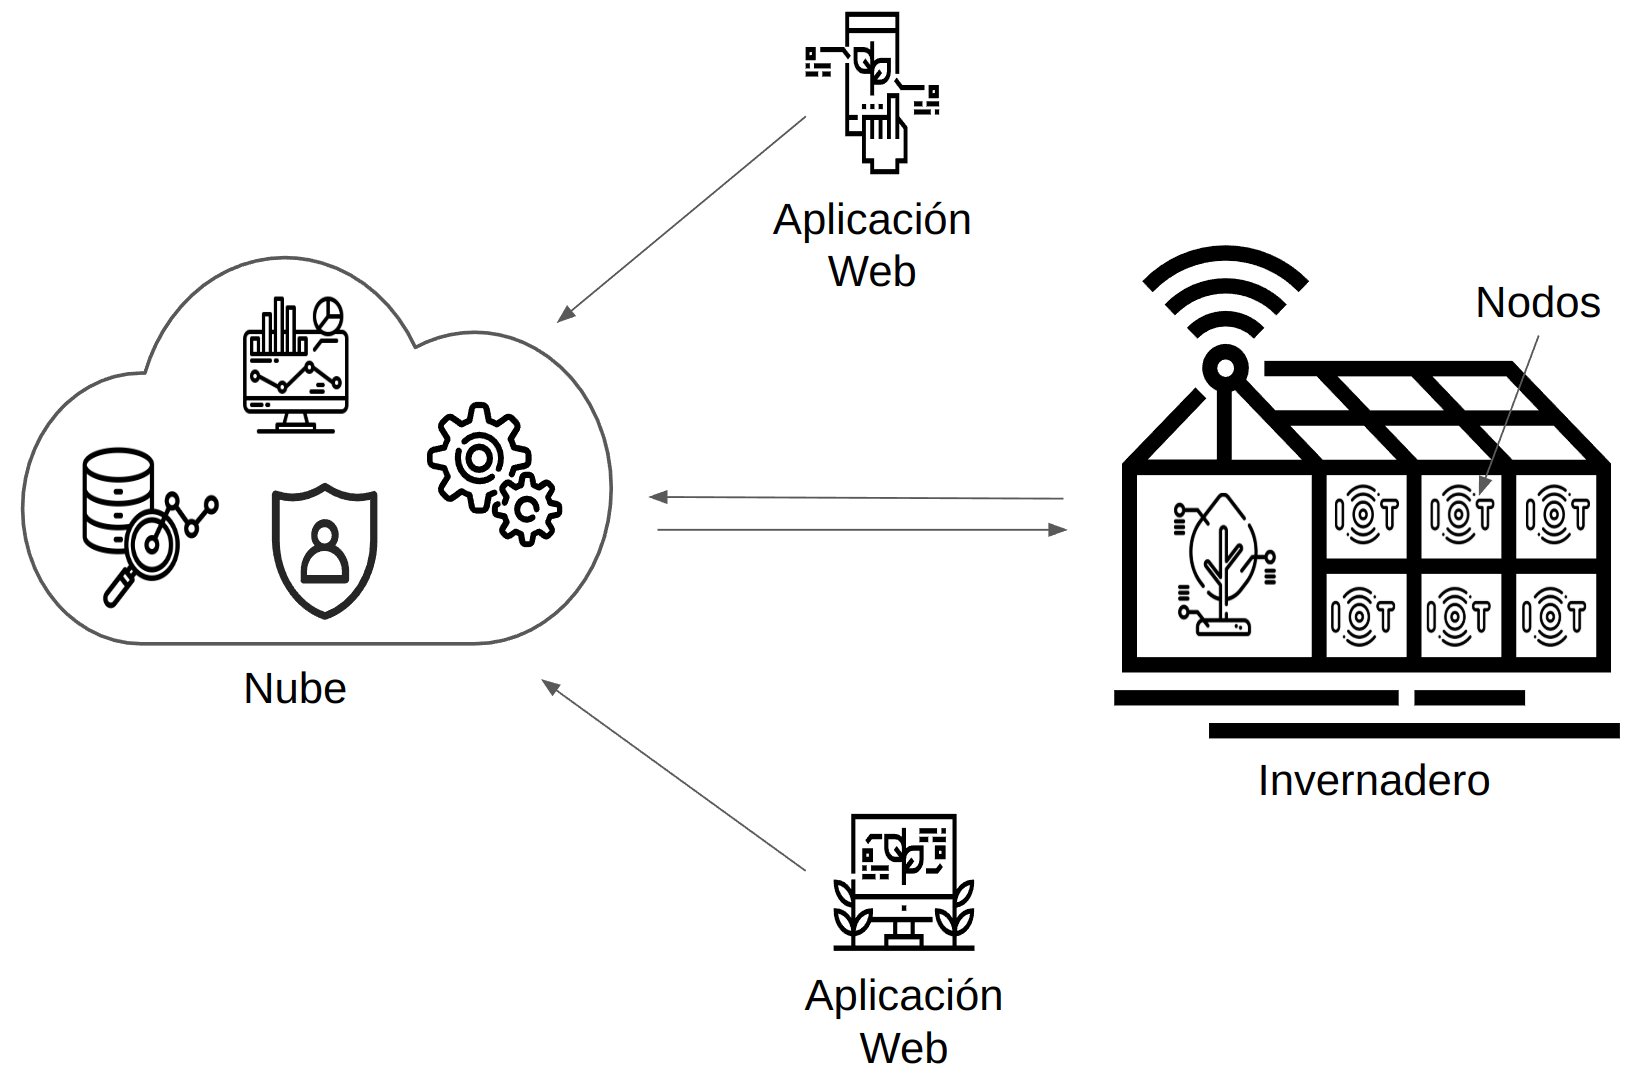
\includegraphics[width=.85\textwidth]{./Images/1.png}
      \caption{Diagrama en bloques del sistema.}
      \label{fig:diagBloques}
\end{figure}

%----------------------------------------------------------------------------------------

\section{Requerimientos}

A continuación, se detallan los requerimientos técnicos asociados a los
diferentes componentes del sistema.

\begin{enumerate}
      \item Requerimientos de los nodos:
            \begin{enumerate}
                  \item Utilizar microcontroladores basados en ESP32.
                  \item Implementar certificados TLS para seguridad en las comunicaciones.
                  \item Permitir conexión Wi-Fi.
                  \item Identificador único por nodo dentro del sistema.
                  \item Configuración remota del intervalo de envío de datos.
                  \item Los nodos sensores deben transmitir al servidor IoT:
                        \begin{enumerate}
                              \item Nodos ambientales: temperatura ambiente, humedad relativa, presión atmosférica, nivel de
                                    luminosidad y nivel de $CO_2$.
                              \item Nodos de solución nutritiva: valores de pH (potencial de Hidrógeno),
                                    conductividad eléctrica (CE) y TDS (del inglés, \textit{Total Dissolved Solids}); nivel y
                                    temperatura de la solución.
                              \item Nodos de consumos: agua, nutrientes y energía eléctrica.
                        \end{enumerate}
                  \item Los nodos actuadores deben transmitir al servidor IoT:
                        \begin{enumerate}
                              \item Configuración remota de parámetros por cada canal.
                              \item Reporte del estado de cada canal.
                        \end{enumerate}
                  \item Los nodos actuadores deben recibir desde el servidor IoT:
                        \begin{enumerate}
                              \item Comandos de activación/desactivación remota de canales.
                        \end{enumerate}
            \end{enumerate}

      \item Broker MQTT:
            \begin{enumerate}
                  \item Soportar conexiones cifradas mediante TLS.
                  \item Poseer comunicación bidireccional (publicación/suscripción).
                  \item Implementar QoS (del inglés, \textit{Quality of Service}) para garantizar entrega de
                        mensajes.
            \end{enumerate}

      \item Frontend (aplicación web)
            \begin{enumerate}
                  \item Interfaz intuitiva y responsiva (accesible desde móviles y escritorio).
                  \item Autenticación de usuarios mediante credenciales.
                  \item Realización de las operaciones CRUD (Crear, Leer, Actualizar, Eliminar).
                  \item Visualización en tiempo real de datos de sensores y actuadores.
                  \item Envío remoto de comandos y configuraciones.
                  \item Acceso a datos históricos mediante gráficos y tablas.
                  \item Tablero interactivo para monitoreo y control centralizado.
            \end{enumerate}

      \item Backend:
            \begin{enumerate}
                  \item Tener conexiones seguras mediante TLS.
                  \item Implementar JWT (del inglés, \textit{JSON Web Token}).
                  \item Realizar la persistencia de los datos.
                  \item Soportar métodos HTTP (CRUD y reportes), WebSockets (datos en tiempo real)
                        y MQTT (interacción con dispositivos).
            \end{enumerate}

      \item Requerimientos de documentación:
            \begin{enumerate}
                  \item Se entregará el código del sistema, que incluye todos los componentes
                        desarrollados (sensores, actuadores, broker MQTT, frontend, backend y API).
                  \item Se entregarán las guías y diagramas de instalación, configuración y operación.
            \end{enumerate}
\end{enumerate}

